\newpage
\section{Методы бинарной классификации признаков}

Детектирование лиц на изображении относится к задачам бинарной классификации. Пусть $X = \{x_i\}$ -- множество произвольных областей изображения, $Y = \{−1, 1\}$ -- множество меток классов, $k \in K$ -- алгоритмы бинарной классификации, тогда процесс классификации областей может быть записан следующим образом:

\begin{gather}
X\xrightarrow{k}Y
\end{gather}

Предположим, что для некоторых $\hat{x}_j \in \hat{X} \subset X$ известны ответы $\hat{y}_j \in \hat{Y} \subset Y$, $j = 1, \dots, L$. Отображение вида

\begin{gather}
(\hat{X} \times \hat{Y})^L \rightarrow k
\end{gather}
называется алгоритмом обучения классификатора k.

Для оценки производительности классификатора вводится функция потерь $L(k, x)$ -- величина ошибки алгоритма k на элементе x из множества X. При решении задач бинарной классификации часто используется функция потерь от одного аргумента:

\begin{gather}
L(k, x) = L(y \ast k(x))
\end{gather}

где y -- метка класса элемента x.

\subsection{Композиции классификаторов}

Рассмотрим изображение $X$ и функцию $f_i(x)$, где $x$ -- некоторая произвольная область изображения, а $f_i$ -- скалярная функция вычисления признака от заданной области. Согласно представленным в предыдущих разделах описаниям видов признаков, $f_i$ может вычисляться как свертка изображения с одним из вейвлетов
Хаара по формуле (10)(22) или являться i-ым бином гистограммы признаков ЛБШ (19). Применительно к ДКП-2 $f_i$ можно представить как i-ый коэффициент преобразования $F(u, v)$ при фиксированном положении окна.

Набор всевозможных функций вида (25) будем называть множеством слабых (элементарных) классификаторов

\begin{gather}
k_i(x, a_i) = k_i(f_i, x, p_i, \theta_i) = 
  \begin{cases}
    1, \quad p_if_i(x) < p_i \theta_i \\
    -1, \quad \text{иначе}
 \end{cases}
\end{gather}
где $\theta$ -- порог принятия решения, $p \in \{−1, 1\}$ определяет направление знака неравенства, $k_i \in K$, $a_i = \{f_i, p_i, \theta_i\}$ -- набор указанных параметров. Применительно к задаче детектирования лиц на изображениях, множество $K$ можно представить как совокупность независимых детекторов, анализирующих каждую область изображения. Поскольку заранее неизвестно, какие из признаков окажутся наиболее информативными для описания конкретного паттерна лица, то на этапе обучения алгоритма детектирования целесообразно проверить все доступные элементарные детекторы и попытаться сформировать один "сильный" детектор.

Процедура последовательного построения композиции элементарных классификаторов, когда каждый последующий классификатор стремится компенсировать недостатки композиции всех предыдущих, получила название бустинга (boosting). Алгоритм бустинга является жадным алгоритмом -- на каждом шаге, компенсируя ошибку предыдущей композиции, он принимает локально оптимальное решение, будучи уверенным, что итоговое решение будет также
оптимальным. Цель бустинга -- построение композиции $s_D$ слабых алгоритмов $k_i$:

\begin{gather}
s_D(x)=s(k_1(x),k_2(x),\dots,k_L(x))
\end{gather}

Процесс последовательного обучения композиции может иметь следующие критерии останова:
\begin{itemize}
\item построено заданное количество элементарных классификаторов L,
\item достигнута заданная точность на обучающей выборке,
\item достигнутую точность не удается улучшить на протяжении T шагов.
\end{itemize}

Закономерным результатом развития данного подхода стал алгоритм адаптивного бустинга. Количество классификаторов в композиции стало произвольным, а каждый последующий классификатор строится на ошибочных ответах предыдущих (адаптивность), используя одну и ту же базу для обучения. Для алгоритма адаптивного бустинга впервые была доказана теорема бустинга, которая задавала оптимальный способ формирования композиции слабых классификаторов в виде взвешенной суммы.

\subsection{Адаптивный бустинг и метод Виолы-Джонса}

Рассмотрим три модификации алгоритма адаптивного бустинга, применяющихся для построения детектора лиц:
\begin{itemize}
\item Дискретный адаптивный бустинг (Discrete Adaptive Boosting, DAB).
\item Вещественный адаптивный бустинг (Real Adaptive Boosting, RAB).
\item Плавный адаптивный бустинг (Gentle Adaptive Boosting, GAB).
\end{itemize}

Алгоритм DAB был предложен Фройндом и Шапире. При построении композиции классификаторов алгоритмом DAB используются два типа весов: коэффициенты взвешенного голосования классификаторов $c_m \in C$ и веса обучающих сэмплов $w_i \in W$. На каждой итерации алгоритм DAB увеличивает веса тех наблюдений $x_i$, на которых классификаторы чаще ошибаются. Доля решения классификатора в общем голосовании $c_m$ определяется точностью его решений на выборке $X$. Формула взвешенного голосования DAB выглядит следующим образом:

\begin{gather}
s_D(x)=\sum\limits_{m=1}^{M}c_mk_m(x)
\end{gather}

Перед началом итеративного процесса веса объектов полагаются одинаковыми (28). На каждой итерации выполняется перенормировка весов с целью выполнения условия (29).

\begin{gather}
w_i=\frac{1}{N},\quad i = 1, \dots, N
\end{gather}

\begin{gather}
\sum\limits_{i=1}^{N}w_i=1
\end{gather}

Для каждого классификатора из множества K выполняется три шага:
\begin{enumerate}
{\item Сначала на выборке X обучается классификатор $k_m(x, a_m)$ (в более общем случае $k_m = k_m (x, a_m , W))$:

\begin{gather}
k_m=\underset{a_m} {\mathrm{argmax}}\sum\limits_{i=1}^{N}L(y_i w_i k(x_i, a_m))
\end{gather}

}
{\item Затем, рассчитывается ошибка m-го классификатора на всем обучающем множестве.

\begin{gather}
\mathcal{E}_m= \frac{1}{N} \sum\limits_{i=1}^{N} 1_{\{ y_i \neq k_m(x_i) \}}
\end{gather}

Согласно основной теореме бустинга, определяется вес классификатора $k_m$ в финальной композиции:

\begin{gather}
c_m = \frac{1}{2} \ln \dfrac{1-\mathcal{E}_m}{\mathcal{E}_m}
\end{gather}

}
{\item Наконец, обновляются веса для каждого сэмпла из базы обучения. При изменении весов используется экспоненциальная функция потерь: $L(k, x) = e^{-y \ast k(x)}$.

\begin{gather}
w_i = w_i e ^{c_m 1_{\{y_i \neq k_m(x_i)\}}}
\end{gather}

\begin{gather}
w_i = \dfrac{w_i}{\sum_{j=1}^{N}w_j}
\end{gather}

}
\end{enumerate}

RAB является вероятностным обобщением алгоритма DAB. Дискретное множество ответов $Y = \{−1, 1\}$ заменяется на непрерывную оценку $f_m(x)$, знак которой определяет класс распознанного объекта, а модуль -- степень "уверенности" классификатора. Голосование классификаторов задается суммой вкладов $f_m$:

\begin{gather}
s_R(x) = \sum\limits_{m=1}^{M} f_m(x)
\end{gather}

На втором шаге m-ой итерации, после обучения классификатора на выборке X, рассчитывается оценка вероятности положительного класса:

\begin{gather}
p_m(X) = \hat{P}_w(y = 1|x)
\end{gather}

Вклад m-го классификатора в общее решение определяется логит-функцией от вероятности положительного класса:

\begin{gather}
f_m(X) = \frac{1}{2} \ln \dfrac{p_m(x)}{1-p_m(x)}
\end{gather}

На третьем шаге формула обновления весов принимает следующий вид:

\begin{gather}
w_i = w_i e^{-y_i f_m (x_i)}
\end{gather}

Главное отличие алгоритма GAB от RAB -- это способ оценки вероятностей классов, определяющих функции слабых классификаторов. В RAB для этого используется логистическая регрессия (37), а в алгоритме GAB рассчитывается разность между вероятностями двух классов (39).

\begin{gather}
f_m(X)=\hat{P}_w(y=1|x)-\hat{P}_w(y=-1|x)
\end{gather}

В то время как оценка (37) является численно неустойчивой, функция, задаваемая формулой (39), всегда лежит в пределах $[−1, 1]$. Другим отличием является аппроксимация функции потерь: алгоритм RAB использует экспоненциальную оценку, GAB -- квадратичную.

Используя вейвлеты Хаара в качестве признаков для слабых классификаторов, Пол Виола и Майкл Джонс предложили обучать методом адаптивного бустинга сильные алгоритмы и затем выстраивать их в однобокое дерево решений, которое называется каскадом. На каждом уровне каскада сильный классификатор выносит решение, является ли образец искомым паттерном (в нашем случае лицом) или нет (рис. 10).

\begin{figure}[h!]
\centering
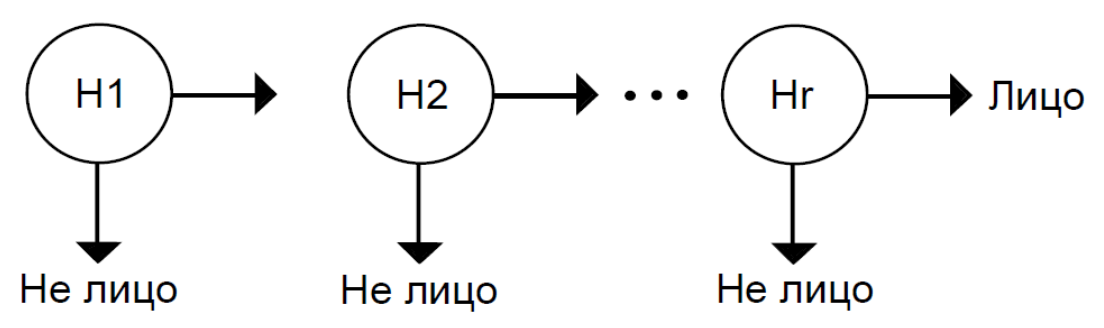
\includegraphics[scale=0.45]{res/pic010}
\caption{Пример вырожденного дерева каскадов}
\end{figure}

Решение каскадного классификатора D может быть записано, как произведение ответов r сильных классификаторов $H_i$:

\begin{gather}
D = \prod\limits_{i=1}^{r} H_i
\end{gather}

Преимущество такого подхода перед одним сильным классификатором объясняется скоростью принятия решений. В качестве эксперимента сильный классификатор, обученный по методу AdaBoost и содержащий 200 признаков, сравнивался с каскадным классификатором, состоящим из 10 уровней по 20 признаков на каждом. В то время как TPR отличался на 2-3\% в пользу сильного классификатора, производительность каскада была почти в 10 раз выше.

\subsection{Смеси гауссовых распределений}

Рассмотрим матрицу X, по столбцам которой расположены вектора признаков изображения. Предполагается, что распределение каждого элемента вектора признаков подчиняется нормальному, поскольку при построении тот подвержен влиянию огромного числа случайных факторов. В качестве генеративного метода, моделирующего характеристики наблюдаемого объекта и среды наблюдения, хорошо зарекомендовали себя смеси гауссовых распределений (СГР). Модель гауссовых смесей может быть записана следующим образом:

\begin{gather}
P(X|\theta) = \sum\limits_{i=1}^{K} a_i \text{Norm}_x[\mu_i,\Sigma_i]
\end{gather}

\begin{gather}
\text{Norm}_x[\mu_i,\Sigma_i]=\frac{1}{(2\pi)^\frac{D}{2} |\Sigma_i|^\frac{1}{2}}e^{-\frac{1}{2}(X-\overline{\mu}_i)^T \Sigma_i^{-1}(X-\overline{\mu}_i)}
\end{gather}

где $X$ -- $D$-мерный вектор случайных величин, $\overline{\mu}_i$ -- вектор математического ожидания, $\Sigma_i$ -- ковариационная матрица, $\alpha_i$ -- веса смеси: $\sum_{i=1}^{N} \alpha_i = 1$, $\theta = [\alpha_i, \overline{\mu}_i, \Sigma_i]$ -- параметры гауссовой смеси, $K$ -- количество гауссоид.

Для построения СГР используется классический EM-алгоритм (Expectation-maximization algorithm), максимизирующий правдоподобие модели на заданных обучающих данных. На E-шаге вычисляется ожидаемое значение функции правдоподобия, при этом скрытые переменные рассматриваются как наблюдаемые (43). На M-шаге рассчитывается оценка максимального правдоподобия, таким образом, увеличивается ожидаемое правдоподобие, вычисляемое на E-шаге. Производится переоценка вектора параметров, используя текущее значение вектора скрытых переменных (44)-(46).

\begin{gather}
\gamma_{nk} = \frac{\alpha_k \text{Norm}_{X_n}[\mu_k,\Sigma_k]}{\sum_{j=1}^{K} \alpha_j \text{Norm}_{X_n}[\mu_k,\Sigma_k]}
\end{gather}

\begin{gather}
\hat{\mu}_k = \frac{1}{N_k} \sum\limits_{n=1}^{N} \gamma_{nk} X_n
\end{gather}

\begin{gather}
\hat{\Sigma}_k = \frac{1}{N_k} \sum\limits_{n=1}^{N} \gamma_{nk} (X_n - \hat{\mu}_k) (X_n - \hat{\mu}_k)^T
\end{gather}

\begin{gather}
\hat{\alpha}_k = \frac{N}{N_k}
\end{gather}

где $N_k = \sum_{n=1}^{N} \gamma_{nk}$, N -- количество элементов обучающей выборки. Пример итеративной сходимости алгоритма показан на рисунке 11.

При обучении модели гауссовых смесей необходимо провести инициализацию параметров модели перед первой итерацией. Не гарантируется нахождение глобального максимума в пространстве данных обучения, таким образом, результат обучения системы в значительной степени зависит от начальных значений. Предположим, что число гауссоид $K$ заранее задано, тогда для инициализации параметров $[\alpha_i, \overline{\mu}_i, \Sigma_i]$ может использоваться случайная инициализация параметров модели, алгоритм $k$-средних, метод главных компонент и др.

\begin{figure}[h!]
\centering
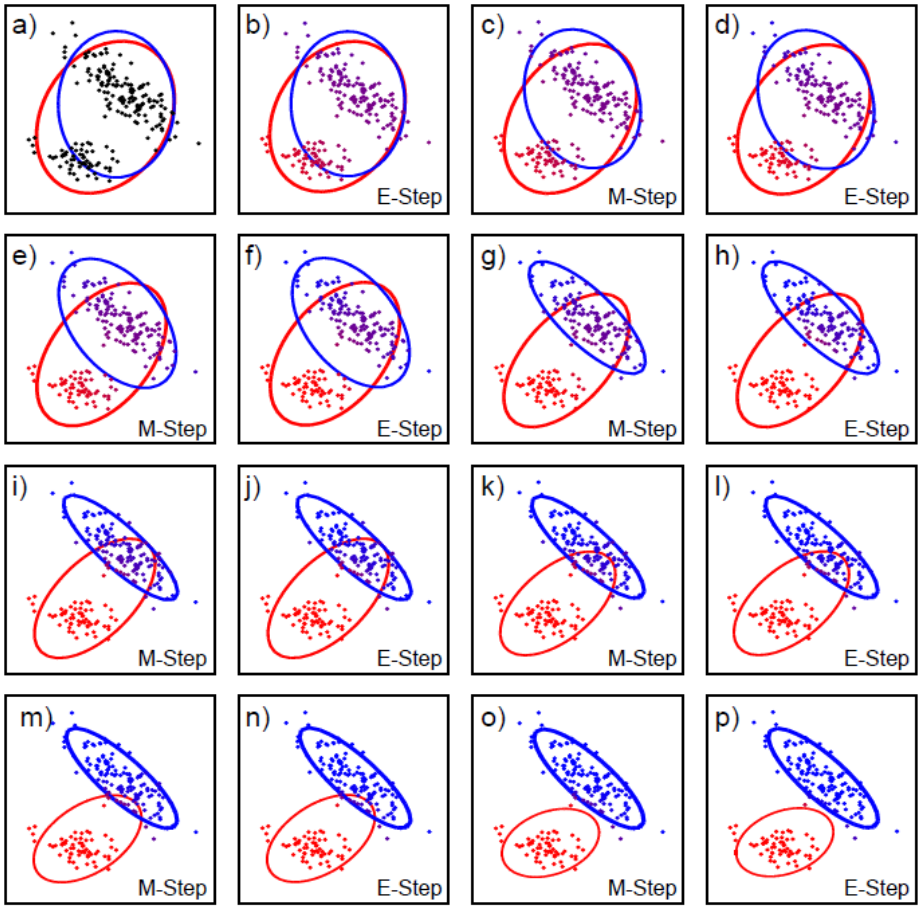
\includegraphics[scale=0.4]{res/pic011}
\caption{a) Исходная модель. b) E-шаг. Для каждой точки плоскости была рассчитана постериорная вероятность, порожденная из каждой гауссоиды (обозначена соответствующим цветом). с) M-шаг. Обновлены среднее, дисперсия и веса каждой гауссоиды согласно постериорным вероятностям Эллипсы отображают расстояние Махаланобиса, их толщина -- вес гауссоиды. d)-t) Череда E- и M-шагов.}
\end{figure}

При обучении СГР-модели важно предупредить случаи, когда эллипсы гауссоид могут превратиться в точку (проблема "схлопывания гауссоид") или покрыть всю выборку. Для предотвращения этого обычно вводят ограничения на элементы дисперсионной матрицы $\Sigma_i$.